
\section*{Общая характеристика работы}

\newcommand{\actuality}{\underline{\textbf{\actualityTXT}}}
\newcommand{\progress}{\underline{\textbf{\progressTXT}}}
\newcommand{\aim}{\underline{{\textbf\aimTXT}}}
\newcommand{\tasks}{\underline{\textbf{\tasksTXT}}}
\newcommand{\novelty}{\underline{\textbf{\noveltyTXT}}}
\newcommand{\influence}{\underline{\textbf{\influenceTXT}}}
\newcommand{\methods}{\underline{\textbf{\methodsTXT}}}
\newcommand{\defpositions}{\underline{\textbf{\defpositionsTXT}}}
\newcommand{\reliability}{\underline{\textbf{\reliabilityTXT}}}
\newcommand{\probation}{\underline{\textbf{\probationTXT}}}
\newcommand{\contribution}{\underline{\textbf{\contributionTXT}}}
\newcommand{\publications}{\underline{\textbf{\publicationsTXT}}}


% Обзор, введение в тему, обозначение места данной работы в
% мировых исследованиях и~т.\:п., можно использовать ссылки на~другие
% работы\cite{Joshi2015}
% % (если их~нет, то~в~автореферате
% автоматически пропадёт раздел <<Список литературы>>). Внимание! Ссылки
% на~другие работы в разделе общей характеристики работы можно
% использовать только при использовании \verb!biblatex! (из-за технических
% ограничений \verb!bibtex8!. Это связано с тем, что одна
% и~та~же~характеристика используются и~в~тексте диссертации, и в
% автореферате. В~последнем, согласно ГОСТ, должен присутствовать список
% работ автора по~теме диссертации, а~\verb!bibtex8! не~умеет выводить в одном
% файле два списка литературы).
% При использовании \verb!biblatex! возможно использование исключительно
% в~автореферате подстрочных ссылок
% для других работ командой \verb!\autocite!, а~также цитирование
% собственных работ командой \verb!\cite!. Для этого в~файле
% \verb!Synopsis/setup.tex! необходимо присвоить положительное значение
% счётчику \verb!\setcounter{usefootcite}{1}!.

% Для генерации содержимого титульного листа автореферата, диссертации
% и~презентации используются данные из файла \verb!common/data.tex!. Если,
% например, вы меняете название диссертации, то оно автоматически
% появится в~итоговых файлах после очередного запуска \LaTeX. Согласно
% ГОСТ 7.0.11-2011 <<5.1.1 Титульный лист является первой страницей
% диссертации, служит источником информации, необходимой для обработки и
% поиска документа>>. Наличие логотипа организации на титульном листе
% упрощает обработку и поиск, для этого разметите логотип вашей
% организации в папке images в формате PDF (лучше найти его в векторном
% варианте, чтобы он хорошо смотрелся при печати) под именем
% \verb!logo.pdf!. Настроить размер изображения с логотипом можно
% в~соответствующих местах файлов \verb!title.tex!  отдельно для
% диссертации и автореферата. Если вам логотип не~нужен, то просто
% удалите файл с логотипом.

{\actuality}

From the birth of the first civilizations to the present, the questions of how
consciousness and reason are organized in man and other living beings continue
to be key for us.  It so happened that their reflection first took place within
the framework of religious and then philosophical paradigms, which in Western
European tradition significantly echoed and complemented each other.

The scientific approach to cognition was formed only relatively recently within
the group of disciplines that include biology, neurophysiology, cognitive
psychology and electrophysiology. Within these disciplines, the key to
understanding the cognitive function of humans and animals in the broadest
sense is the structure of the central nervous system and, in particular, the
brain.

Interestingly, the cognitive mechanisms have not always been associated with
brain function, even within the framework of materialistic description. For
example, Aristotle considered the heart as the source of thought, and the brain
was given only the role of a radiator, cooling the blood. Nevertheless, already
in the era of classical antiquity Galen has formed the idea that it is the
brain that is the source of thought, and thus the tool by which knowledge is
realized.  Then, it took more than one and a half thousand years for the idea
to take root that the study of the central nervous system and its highest
department - the cortex of the large hemispheres - can offer an answer to the
fundamental question" what is the human intellect". To date, there is still no
satisfactory answer to this question, and it will probably not appear soon.
However, in the course of a long and difficult movement towards this Ultima
Thule, our understanding of more applied things revolving around
neurophysiology has been incomparably enriched.   From a practical point of
view, it is difficult to overestimate the importance of understanding the work
of the CNS for medicine, however, not limited to it alone.

Today, along with the general blurring of interdisciplinary boundaries,
neurosciences are increasingly linked to more technical and engineering
disciplines.  For example, in 1943, inspired by the architecture of neural
ensembles of the living brain, McCulloch and Pitts created the first
computational model of the neural network, thus creating a class of machine
learning algorithms so popular today~\cite{McCulloch}. Brain-computer
interfaces, which allow to form a control command based on the electromagnetic
activity of the brain directly, are becoming increasingly popular today, which
opens up completely new prospects for human integration with the machine.

% \section{Модальности изучения активности мозга.}

In this regard, the development of methods related to the study of the
structure and work of the brain, as well as the decoding of the signals
generated by it are of extreme interest today.  At the same time, over the last
hundred years, thanks to a dramatic leap in the development of electronics,
physics and computer science, the set of tools in the hands of a
neurophysiologist has been significantly enriched.  Today, the existing methods
can be divided into invasive and non-invasive from the point of view of the
need for surgery to perform measurements.

The first group includes intracranial encephalography~--- a method in which
electrical potentials are recorded directly from the cortex of the large
hemispheres. Shortcomings and advantages of this approach are obvious. The
former primarily refers to the need for surgery to perform measurements, which
significantly limits the ability of a neurophysiologist to obtain data for the
study.  In practice, such measurements on a person are possible only for
patients who underwent brain surgery in connection with some neurological
disease, usually epilepsy.  During the operation, electrodes registering
electrical activity are placed on the cortex to monitor brain activity after
surgery. It is clear that the number of such data, as well as the possibility
of conducting any complex cognitive experiments on patients who underwent brain
surgery is very limited.  However, the quality of the electrical signal
recorded in the immediate vicinity of its source is incomparably higher than
that obtained by recording the electroencephalogram from the scalp surface.

Non-invasive methods, on the other hand, provide a much more flexible tool for
human brain research due to the lack of need for surgery.  Structural
neuroimaging techniques such as Magnetic Resonance Imaging (MRI), Computed
Tomography (CT) and Diffusion Tensor Imaging (DTV) are used to study the
anatomical organization of the brain and as an auxiliary tool in the analysis
of neural cortical population activity.  They allow non-invasive acquisition of
static three-dimensional images of brain tissue. To study the dynamic activity
of neurons, functional neuroimaging techniques are used, namely, ~---
functional magnetic resonance imaging (fMRI), positron emission tomography
(PET), electroencephalogy (EEG), and magnetic encephalography (MEG).

Only the last two methods measure brain electrical activity directly, while
fMRI and PET measure local blood flow, which changes relatively slowly,
significantly limiting the temporal resolution of these methods.  Thus, for EEG
and MEG, the temporal resolution is $\approx$ 1ms, and methods that measure
local blood flow allow only processes with characteristic times of about one
second and slower. At the same time, oscillatory electrophysiological processes
generated by brain tissue have characteristic times from 0.1 seconds and
faster~\cite{buzsaki}. Thus, among all the analysis tools available today,
\emph{ only EEG and MEG allow non-invasive recordings of relatively fast
electrophysiological activity of the brain}, which makes them an indispensable
tool for studying \emph{oscillations} and their \emph{synchronization} in the
human brain.

% \section{Осцилляции и их роль в обмене информацией между популяциями нейронов.}

The ability to generate oscillations or rhythmic current activity is an
essential feature of neural populations. The nature of the emerging rhythms, as
well as their functional purpose, remain a subject of study today, and there is
no uniform, accepted by all viewpoint on this issue. However, the hypothesis
that oscillations generated by different neural populations serve as a
mechanism allowing various functionally specific areas of the brain to
selectively exchange information with each other is widely accepted. In other
words, it is assumed that oscillations are responsible for the \emph{functional
integration} processes.
%~\cite{TODO}.
According to existing conceptions, functional integration of neural ensembles
is carried out by synchronization of oscillations generated by these ensembles.
At the same time, areas of the cortex, where rhythmic activity is synchronized,
are able to transmit information more efficiently, while desynchronized areas,
on the contrary, cease to exchange signals. This idea of organizing effective
channels for information transfer between neural ensembles due to
synchronization was named in the literature as <<communication through
coherence>>~\cite{Fries2015}. In brief, oscillation synchronization is the
mechanism that allows for the dynamic linking of functionally specific brain
regions in a network to perform a specific cognitive task. The study of such
networks, which arise and decay in the process of solving certain cognitive
tasks in the brain, is now one of the central topics in the study of brain
activity, both in typical development and pathology~\cite{varela, baker,
ossadtchi, Bastin2017},~\cite{Alamian_front2017, Alamian_clin2017}.  From the
point of view of research into such networks, the concept of \emph{functional
connectivity} is distinguished, meaning statistical regularities in
simultaneous activation (in the broadest sense) of various brain regions.
%~\cite{TODO}.
At the same time, the conclusion that these brain regions worked synchronously
is based on the calculation of a certain metric reflecting the degree of
similarity of measured (or mathematically recovered) signals in these areas.
Such metrics are called \emph{measures of connectivity}.

Much in the field of functional connectivity has been done with the use of fMRI
technology, but the aforementioned limitation of fMRI in the form of poor
temporal resolution makes electrophysiological methods of measurement
irreplaceable in connectivity analysis. Magnetoencephalography occupies a
special place, which combined with methods of signal recovery on the cortex due
to the higher accuracy of the forward model compared to the EEG provides  a
unique combination of less than a centimeter resolution in space and
millisecond resolution in time~\cite{hamalainen, Baillet, Gross2013}.


% \section{Существующие методики поиска синхронных осцилляций.}

% {\progress}
In general, the assessment of connectivity on the basis of non-invasive
electrophysiological data is a complex engineering problem, on which the
scientific community has already spent a lot of effort.  Over the past few
decades, many methods for estimating functional connectivity have been
developed and tested from standard approaches that include measures of signal
synchronization in the time and frequency domain (such as correlation and
coherence), to more sophisticated, often non-linear measures of
connectivity~\cite{Marzetti2008, Schoffelen2009, Colclough2015, kaminski,
greenblatt_conn, hillebrand, imcoh, Lachaux1999, env_corr, Brookes2012,
Hillebrand2012, PLI, wPLI, Chella2015, Chella2016, Wibral2011, Ioannides2000}.
None of the proposed measures, with their advantages and disadvantages, is,
however, universal due to the continuing technical
difficulties~\cite{Colclough2016, Bastos2016}.

One of the most significant problems encountered when evaluating functional
connectivity is the so-called \emph{signal leakage}, which is explained by the
fact that the inverse problem for the EEG/MEG is ill-posed. In practice, this
means that having a limited set of measurements it is impossible to
unambiguously restore the configuration of the sources that generated the
signal. This, in turn, means that it is impossible to completely unmix the
signals recorded by the sensors,~--- signals from other sources will
inevitably be mixed in each of the recovered ones. Consequently, all
recovered signals will be to some extent similar to each other, even if the
original signals showed no sign of synchronization. Therefore, the connectivity
measures, being measures of similarity of signals, will show overestimated
values. As a result, there is a problem of distinguishing between true
synchronization and the one that is caused by fundamental constraints of
noninvasive electrophysiology.

The first attempt to solve this problem was made in 2004 in the article by G.
Nolte~\cite{imcoh}, in which the authors propose to use as a measure of
connectivity a value called an imaginary part of coherence.  To do this, each
signal must first be transformed into a frequency domain, then for each pair of
signals, the coherence function must be computed, and finally the imaginary
part of coherence must be taken from the obtained value.  The idea behind this
method of evaluating connectivity is that the imaginary part of the coherence
has a non-zero value only for signals with a non-zero phase difference, while
the leakage effect always manifests itself as a false synchronization with zero
phase delay, thus contributing only to the real part of coherence. Indeed, this
approach significantly increases the robustness of the method to signal
leakage. However, since the coherence function is normalized by the estimated
signal power (which, being purely real values, are subject to the influence of
the signal leakage) the final estimates of connectivity on the imaginary part
of the coherence also, albeit to a lesser extent, spoilt by the effect of
leakage.

This detail was brought to Stam's attention in 2007 in his article~\cite{PLI}.
Stam suggested to use the average value of the phase difference sign of the two
signals instead of an imaginary part of coherence to evaluate synchronization.
Such a measure is very similar to the imaginary part of coherence, but the
normalization (hidden in the operation of taking the imaginary part sign) is
now done only by purely imaginary values, which do not depend on the signal
leakage. Stam called his measure the phase lag index (PLI).

The next step in the evolution of the chain of methods based on the idea of an
imaginary part of coherence is a measure called a weighted phase lag index
(wPLI). It was described by Vinck and co-authors in his 2011 article. The
motivation for developing the new connectivity measure was the fact that the
PLI measure proved to be too unstable with respect to noise. The main drawback
of the phase lag index, as well as its advantage over the imaginary part of the
coherence, lies in the operation of taking the sign.  The fact is that for
noise sources randomly changing phase difference sign has too great an impact
on measurements. To get rid of this shortcoming, Vinck suggested weighing the
phase difference sign by the amplitude of the imaginary part of the
corresponding cross-spectral coefficients. Thus, the contribution from noise
sources of small amplitude is small, which makes the measure more stable.

The family of connectivity measures based on the imaginary part of coherence is
not limited to the three approaches outlined. A similar idea, but from a
slightly different angle, was applied in the article~\cite{Hipp2012}. In this
article, the authors use the correlation of envelopes of two narrowband signals
as a measure of synchronization. The problem of signal leakage is solved in
following way: two time series are reconstructed on the cortex, then one of
them is projected orthogonally to the second, after which the envelopes are
calculated and the correlation coefficient between them is obtained.  This
approach based on orthogonalization of time series turns out to be equivalent
to taking an imaginary part of the corresponding cross-spectral coefficient.


% TODO: Еще можно написать про wedge music

All of the outlined methods, based on the imaginary part of coherence, however,
have one significant drawback, namely ~--- all of them are not sensitive to
zero phase lag synchronization. As mentioned above, taking an imaginary
coherence part is equivalent to removing the zero phase lag synchronization
data. Practically, this means not only that it is impossible to detect networks
synchronized with zero phase delay, but also a poor signal-to-noise ratio (SNR)
for networks with low phase delay. Moreover, the closer this phase delay is to
zero, the worse the SNR for a single pair of sources.  Conversely, the closer
the phase difference between two signals to $\pi / 2$, the higher the SNR
value.

Clearly, this uneven distribution of the method's detector characteristics over
phase delays limits the researcher's capabilities.  This fact is aggravated by
the fact that zero phase synchronization seems to be a widely represented
phenomenon in the organization of oscillatory brain activity, ~\cite{roelfsema,
Singer1999, Engel2001}, which can be explained by the presence of a common
input for two nodes of the network, or by their bidirectional interactions,
~\cite{rajagovindan}.

For this reason, non-invasive electrophysiology nowadays has an acute need for
a connectivity measuring instrument that, on the one hand, will be resistant to
the signal leakage effect and, on the other hand, will be able to detect
networks for the entire spectrum of phase delays.


An attempt to create such method was made in 2015 in the
article~\cite{Wens2015}. In this article, the authors used a fundamentally
different approach to combat the effect of the signal leakage.  The idea of
this method is to use information about the mutual location of signal sources
and sensors to construct specific spatial filters that allow us to clear one
source from a signal that came from another source for subsequent measurement
of any synchronous index. The authors suggested using the correlation of
envelopes as such an index. The structure of the proposed method is as follows
in more details. First, the signals on the sensors are used to restore the
signals on the sources.  Then, one of the sources is fixed on the cortex.  All
other sources are spatially filtered from the activity that leaked from the
fixed source.  Then, the correlation of envelopes between the fixed source and
all other sources is measured.  To get the connectivity value for each pair of
sources, you need to repeat the procedure by selecting each of the remaining
sources as a fixed source.  Finally, since the resulting connectivity matrix is
generally asymmetric, the connector values for the $(i,j)$ and $(j,i)$ pairs
are averaged. Such heuristics has been named by the authors of the article as
geometric correction scheme (GCS).

GCS method conceptually was a serious advance, as now it is possible to detect
networks with small phase shifts, remaining (at least in theory) outside the
influence of the signal leakage effect.  In reality, however, this correction
method only partially eliminates this effect, since it does not take into
account leakage from third sources when assessing connectivity. As an example,
we can consider a situation where there are three powerful sources, no two of
which have been synchronized.  In this setting, despite the lack of
synchronization, the GCS method will give high Connectivity values for all
three pairs of links, because although for each pair the correction will clear
the signals from the leakage into each other, the signal from the third source,
leaking into each source of the pair, will create a common component in the
recovered sources.  As a result, the connectivity we measure for source pairs
that are not synchronous, after the geometric correction for the source pair,
will actually reflect the degree of leakage from the third source into each
signal from the pair. Clearly, if the third signal is close to the first two,
the leakage effect will be quite significant. As a result, for a large number
of active sources, even a cleaned signal is extremely polluted, which
significantly limits the applicability of GCS to practical tasks.



Thus, \emph{ there is still no method for estimating connectivities, which
allows reliable detection of networks with low phase lags and at the same time
free from the signal leakage effect}.


% \section{Оценивание функциональной коннективности в условиях некорректности обратной задачи М/ЭЭГ.}\label{sec:connectivity_and_ill_posedness}

Modern practice of using conectivity measures in neurophysiological studies in
the vast majority of cases follows one of two possible schemes.  The first
scheme assumes studying of neurophysiological effect in \emph{sensor space},
i.e. the measure of connectivity chosen by the researcher is applied directly
to signals recorded by electrodes.  The second variant assumes transition to
source space~--- first, possible sources of recorded electrophysiological
activity on the cortex are estimated, and then this or that measure of
connectivity is applied to these sources.

Obviously, the first option allows you to make only a very rough assessment of
the localization of nodes of the restored networks, so it is often used only as
a first approximation to the result.  More interesting, though more complex
conceptually and more computationally intensive, is the second option, which
first evaluates the signal on the sources and then considers a measure of
connectivity.

Evaluation of sources in noninvasive electrophysiology is an ill-posed inverse
problem~\cite{Hamalainen1993}: its solution could not be unambiguously
determined. In other words, any electrophysiological measurements made with a
limited set of sensors can be explained by the infinite number of
configurations of electromagnetic activity sources located on the cortex. The
vast majority of such configurations would be absurd in terms of physiology.
Among the infinite array of solutions, it is necessary to choose one that on
the one hand explains the observations well, and on the other hand ~---
corresponds to the existing concepts of brain physiology.

Therefore, the solution of the inverse problem in noninvasive electrophysiology
always requires the introduction of additional a priori information about the
solution structure into the model. Not every method of solving the inverse
problem can explicitly specify the point at which an additional assumption
about the solution structure is made, but most of such methods (for example,
~\cite{Hamalainen1994, Uutela1999, Pascual-Marqui1994, Pascual-Marqui2002}) can
be described in terms of Tikhonov regularization~\cite{tikhonov}, which allows
to reduce the solution search task to minimization of the two-member
functional: the first one~--- how well the solution explains the measured
signal, the second one~--- how well it corresponds to the class of solutions
that we consider <<physiological>>. However, formalization of the
<<physiological>> concept can involve a wide range of different assumptions
about the structure of the solution~--- from the natural requirement of
continuity in space and time (as in MNE,~\cite{Hamalainen1994}) to information
about the anatomical structure of the brain.

Source estimation in this setting is optimal from the point of view of
minimization of the selected functional, but in the synchronous oscillations
search task, source estimation is not an end in itself. Optimality of this
estimation does not guarantee optimal estimation of sufficient statistics of
synchronicity in the source space.

The two-step procedure for assessing connectivities generally provides
suboptimal results in terms of evaluating the relevant statistics.
% Ситуация здесь может быть улучшена рассмотрением порождающих моделей для этих статистик статистик.
% В данной работе такой подход изложен в применении к матрице \emph{кросс-спектральной плотности},
% являющейся достаточной статистикой для оценки фазовой синхронности в
% пространстве источников \cite{cross_sufficient}.

Optimal evaluation of the synchrony statistics in source space by observations
requires consideration of generative models with formulation of a priori
assumptions for networks instead of those for sources. In particular, it would
be desirable to find such solutions to the inverse problem that explain the
measurements by \emph{minimum set of networks}. The motivation for this
approach lies in the well-known principle of the Occam Razor~--- the
explanation of the observed data should be as simple as possible. It is known
that solutions of this type, i.e. those in which the number of individual
structural elements explaining the data is minimal, are implemented using
sparse regularization. However, it is not quite clear how to introduce such
regularization in the framework of a two-step procedure.



 % \ifsynopsis
% Этот абзац появляется только в~автореферате.
% Для формирования блоков, которые будут обрабатываться только в~автореферате,
% заведена проверка условия \verb!\!\verb!ifsynopsis!.
% Значение условия задаётся в~основном файле документа (\verb!synopsis.tex! для
% автореферата).
% \else
% Этот абзац появляется только в~диссертации.
% Через проверку условия \verb!\!\verb!ifsynopsis!, задаваемого в~основном файле
% документа (\verb!dissertation.tex! для диссертации), можно сделать новую
% команду, обеспечивающую появление цитаты в~диссертации, но~не~в~автореферате.
% \fi

% Этот раздел должен быть отдельным структурным элементом по
% ГОСТ, но он, как правило, включается в описание актуальности
% темы. Нужен он отдельным структурным элементом или нет ---
% смотрите другие диссертации вашего совета, скорее всего не нужен.

Having in mind all the above, it can be concluded that today the procedure for
assessing connectivity on the basis of non-invasive electrophysiological data
on the one hand is still poorly developed and needs improvement (it is no
coincidence that new methodological articles on the topic of assessing
connectivities are regularly published), and on the other hand is a key tool
for modern neurophysiology, following the shift of emphasis in the study of the
brain from the activation of its individual areas to the interaction between
them.

{\aim} 
The purpose of this study is, therefore, to develop a method for estimating connectivity that

\begin{itemize}
        \item allows to estimate phase synchrony in conditions of mutual signal leakage
        \item is sensitive to networks with low phase lags
        \item optimal in terms of evaluating sufficient statistics for connectivity
        \item is capable of taking into account a priori information on the organization of phase synchronies.
        \item not sensitive to network level signal leaks
\end{itemize}
as well as its validation in application to simulated MEG data.

In order to achieve the set goal it was necessary to solve the following tasks {\tasks}:
\begin{enumerate}
  \item Develop a method of signal leakage removal.
  \item Explore the properties of signal cleaning techniques for networks with small and large phase shift; compare with the techniques described in the literature.
  \item Develop a methodology for optimal evaluation of sufficient statistics for phase synchronicity.
  \item Implement an estimation algorithm allowing the use of sparse regularization.
  \item Develop code for numerical solution of the task of non-convex optimization
  \item Develop a method to visualize the found networks.
  \item Develop a methodology for generating data simulating brain activity.
  \item Compare the detector characteristics of the developed method on simulated data on standard metrics (AUC-ROC, AUC-Pre-Rec)
\end{enumerate}


{\novelty}
\begin{enumerate}
  \item For the first time, the problem of connectivity estimation was considered in the source pair space
  \item For the first time it was demonstrated that it is possible to clean the signal from the leakage effect by means of orthogonal projection operation.
  \item For the first time the criterion of optimal signal leakage filtering for phase synchronization evaluation was formulated.
  \item For the first time, the task of evaluating the cross-spectral density matrix in the source space was solved by the global optimization method.
\end{enumerate}

{\influence} 
Theoretical importance is determined by the fact that for the first time was
proposed an approach to combat the problem of signal leakage through the
vectorization of the generating model of the cross-spectrum, as well as through
methods of optimal filtering and global optimization.

Practical significance is based on the fact that the developed set of
algorithms provides a new tool in the hands of a
researcher-electrophysiologist. This tool makes it possible to study
interactions of cortical structures, previously available for study only by
invasive methods.

{\methods}
Studies are based on the theory of inverse problems, the theory of estimation,
methods of digital signal processing, optimal filtration, global optimization
of non-convex functions, as well as work on methods of connectivity estimation
in electrophysiology.

{\defpositions}
\begin{enumerate}
  \item A method has been developed that allows detecting phase-linked sources with near-zero phase delays from non-invasive MEG records. The essence of the method is to build a spatial filter that operates in the space of vectorized matrices of cross-spectral power density, which allows you to suppress the contribution of members responsible for the signal leakage effect that masks information about the interaction with the near-zero phase.
  \item The optimality of the proposed filter in terms of removing the contribution of third sources to the phase connectivity assessment for a fixed network is shown.
  \item Based on the global IrMxNE optimization method and the proposed filter, a leak-resistant method was developed at the networks and sources levels. The former is provided by the sparse properties of the IrMxNE method, the latter~--- by the properties of the developed filter.
\end{enumerate}

{\reliability} 
The reliability of the obtained results is provided by theoretical
calculations, results of numerical modeling, comparison with other methods of
phase connectivity estimation as well as validation of the developed method on
real data.

{\probation}

The main results of the present work were reported on:
\begin{enumerate}
    \item International conference ``Methodological problems of cortex regions functional synchronisation assessment based on MEG/EEG data'',\\
      Тема: \emph{Globally-optimized power and shift invariant imaging of coherent sources (GO-PSIICOS)}\\
      Moscow, Russia, 2015.
    \item International conference ``Brain Connectivity Workshop 2015'', \\
        Title: \emph{GO-PSIICOS (Globally-Optimized Power and Shift Invariant Imaging of Coherent Sources)},\\
        San Diego, USA, 2015.
    \item International conference ``Biomag 2016'', \\
        Title: \emph{Power and shift invariant imaging of coherent sources by MEG data},\\
        Seoul, South Korea, 2016.
    \item International conference ``Biomag 2018'', \\
        Title: \emph{Oblique projection for phase shift invariant imaging of coherent sources},\\
        Philadelphia, USA, 2018.
    \item International conference ``Biomag 2018'', \\
        Title: \emph{NeuroPycon: A python package for efficient multi-modal brain network analysis},\\
        Philadelphia, USA, 2018.
\end{enumerate}



{\contribution}
All results presented in the dissertation were obtained personally by the
author. In preparing articles and reports, the author relied on the assistance
of co-authors and the scientific adviser.

\ifnumequal{\value{bibliosel}}{0}{% Встроенная реализация с загрузкой файла через движок bibtex8
    \publications\ Основные результаты по теме диссертации изложены в XX печатных изданиях,
    X из которых изданы в журналах, рекомендованных ВАК,
    X "--- в тезисах докладов.%
}{% Реализация пакетом biblatex через движок biber
%Сделана отдельная секция, чтобы не отображались в списке цитированных материалов
    \begin{refsection}[vak,papers,conf]% Подсчет и нумерация авторских работ. Засчитываются только те, которые были прописаны внутри \nocite{}.
        %Чтобы сменить порядок разделов в сгрупированном списке литературы необходимо перетасовать следующие три строчки, а также команды в разделе \newcommand*{\insertbiblioauthorgrouped} в файле biblio/biblatex.tex
        \printbibliography[heading=countauthorvak, env=countauthorvak, keyword=biblioauthorvak, section=1]%
        \printbibliography[heading=countauthorconf, env=countauthorconf, keyword=biblioauthorconf, section=1]%
        \printbibliography[heading=countauthornotvak, env=countauthornotvak, keyword=biblioauthornotvak, section=1]%
        \printbibliography[heading=countauthor, env=countauthor, keyword=biblioauthor, section=1]%
        \nocite{%Порядок перечисления в этом блоке определяет порядок вывода в списке публикаций автора
                PSIICOS, Neuropycon, Visbrain, Alamian_front2017, Alamian_clin2017%
        }%
        \publications\ Основные результаты по теме диссертации изложены в~\arabic{citeauthor}~печатных изданиях,
        \arabic{citeauthorvak} из которых изданы в журналах, рекомендованных ВАК,
        \arabic{citeauthorconf} "--- в~тезисах докладов.
    \end{refsection}
    \begin{refsection}[vak,papers,conf]%Блок, позволяющий отобрать из всех работ автора наиболее значимые, и только их вывести в автореферате, но считать в блоке выше общее число работ
        \printbibliography[heading=countauthorvak, env=countauthorvak, keyword=biblioauthorvak, section=2]%
        \printbibliography[heading=countauthornotvak, env=countauthornotvak, keyword=biblioauthornotvak, section=2]%
        \printbibliography[heading=countauthorconf, env=countauthorconf, keyword=biblioauthorconf, section=2]%
        \printbibliography[heading=countauthor, env=countauthor, keyword=biblioauthor, section=2]%
        \nocite{PSIICOS, Neuropycon, Visbrain, Alamian_front2017, Alamian_clin2017}%vak
        \nocite{}%notvak
        \nocite{confbib1}%conf
    \end{refsection}
}
% При использовании пакета \verb!biblatex! для автоматического подсчёта
% количества публикаций автора по теме диссертации, необходимо
% их~здесь перечислить с использованием команды \verb!\nocite!.
 % Характеристика работы по структуре во введении и в автореферате не отличается (ГОСТ Р 7.0.11, пункты 5.3.1 и 9.2.1), потому её загружаем из одного и того же внешнего файла, предварительно задав форму выделения некоторым параметрам

%Диссертационная работа была выполнена при поддержке грантов ...

%\underline{\textbf{Объем и структура работы.}} Диссертация состоит из~введения, четырех глав, заключения и~приложения. Полный объем диссертации \textbf{ХХХ}~страниц текста с~\textbf{ХХ}~рисунками и~5~таблицами. Список литературы содержит \textbf{ХХX}~наименование.

%\newpage
\section*{Contents}
Во \underline{\textbf{введении}} обосновывается актуальность
исследований, проводимых в~рамках данной диссертационной работы,
приводится обзор научной литературы по изучаемой проблеме,
формулируется цель, ставятся задачи работы, излагается научная новизна
и практическая значимость представляемой работы.


\underline{\textbf{First chapter}}

В первой главе мы формулируем методологический базис для исследования коннективности
при помощи МЭГ и ЭЭГ, основанный на известных и широко используемых на сегодняшний
день методах решения обратной задачи и оценки коннективности для МЭГ и ЭЭГ.

Мы начинаем с описания биологических механизмов обмена информацией
между популяциями нейронов и описываем гипотезу взаимодействия через когерентность,
согласно которой для эффективного взаимодействия популяции нейронов должны работать
в режиме когерентных осцилляций. Далее мы вводим формальное определение функции когерентности
двух сигналов, порождаемых мозговыми источниками.

Так как для неинвазивных методов (МЭГ и ЭЭГ) мы не имеем прямого доступа к сигналам,
порождаемым корой, мы рассматриваем физические механизмы генерации сигнала МЭГ/ЭЭГ,
которые позволяют нам сформулировать понятие прямого оператора~--- линейного соответствия,
между сигналом, порождаемым корой и сигналом, который регистрируют сенсоры. Прямой
оператор позволяет нам сформулировать порождающую модель для данных неинвазивной электрофизиологии.

Далее на основании порождающей модели мы описываем группу методов решения обратной
задачи и основанных на ней методах оценки коннективности в пространстве источников,
которые составляют методологическую базу для предложенного нами метода оценки
коннективностей.


 % картинку можно добавить так:
% \begin{figure}[ht] 
 %  \centering
 %  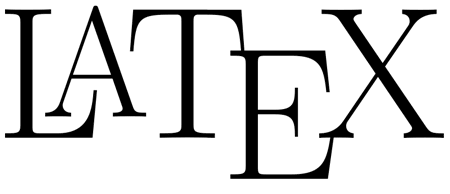
\includegraphics [scale=0.27] {latex}
 %  \caption{Подпись к картинке.} 
 %  \label{img:latex}
% \end{figure}

% Формулы в строку без номера добавляются так:
% \[ 
%   \lambda_{T_s} = K_x\frac{d{x}}{d{T_s}}, \qquad
%   \lambda_{q_s} = K_x\frac{d{x}}{d{q_s}},
% \]

\underline{\textbf{Second chapter}}

In the second chapter we again consider the generative model of the MEG/EEG
signal to formulate the generative model of the cross-spectral density matrix
(cross-spectrum) on its basis. The structure of the cross-spectrum generative
model allows us to explicitly point to the constituents responsible for the
signal leakage effect in the recorded data~--- the effect, which
significantly complicates the evaluation of functional connectivity and masks
the synchronization with low phase lags.


Для удаления источников протечки сигнала мы векторизуем порождающую модель
кросс-спектра и строим оператор ортогональной проекции, который позволяет
подавить вклад нежелательных слагаемых в силу особенной пространственной
структуры трех типов слагаемых, входящих в порождающую модель кросс-спектра:
слагаемых, порождающих протечку сигнала, слагаемых, несущих информацию о
взаимодействии источников с малыми фазовыми сдвигами и слагаемых, несущих
информацию о взаимодействии источников с фазовыми сдвигами, близкими к $\pi/2$.
Для описания пространственной структуры этих слагаемых мы вводим понятие
2-топографии.  Предложенная операция проекции является основной для группы
методов, представленных в данной диссертации

Далее мы обобщаем операцию проекции на модели со свободной ориентацией диполя и
формулируем авторский метод поиска сетей в пространстве источников (PSIICOS).

Затем предложенный метод мы рассматриваем с точки зрения оптимальной
фильтрации, вводя формальное определение взаимной протечки сигнала для двух
узлов сети в пространстве источников.  Мы получаем, что предложенная проекция
порождает пространственные фильтры в пространстве 2-топографий, которые
минимизируют взаимную протечку сигнала для двух точек коры.

Построенные нами фильтры мы изучаем с точки зрения пространственной смещенности
оценки и предлагаем схему нормировки, которая приводит к несмещенной оценке.
Модификацию метода PSIICOS с такой нормировкой фильтров мы называем PSIICOS
Unbiased.

Полученный таким образом метод пространственной фильтрации позволяет
локализовать сети имеющиеся сети, однако он не дает возможности отсечь
ситуацию, когда реальных взаимодействий нет. Причиной тому служит отсутствие
нормировки для оцениваемой метрики силы взаимодействия источников и как
следствие невозможность выбора объективного порога.  Чтобы справиться с этим
обстоятельством, мы формулируем метод нормировки оцененных кросс-спектральных
коэффициентов с учетом эффектра протечки сигнала. Полученный метод мы называем
PSIICOS Normalized.


Чтобы справиться с эффектом протечки сигнала на уровне сетей, мы описываем
известный в литературе метод оценки со смешанной нормой, который порождает
разреженные по пространству решения, и модифицируем его для работы в
пространстве сетей с применением предложенной проекции. Полученный метод мы
называем GO-PSIICOS.


\underline{\textbf{Third chapter}}

Для валидации предложенного метода проекции в этой главе мы сравниваем PSIICOS
с набором алгоритмов, широко используемых в нейронаучной литературе на наборе
экспериментов-симуляций.  Результаты численного моделирования показывают
превосходящие детекторные характеристики PSIICOS по сравнению с остальными
методами, использованными для сравнения, в особенности для сетей с малыми
фазовыми задержками.

Далее на основе симуляционных данных мы исследуем свойства метода PSIICOS.\@ В
частности, мы показываем, что детекторные характеристики алгоритма
действительно показывают равномерно высокое качество решений для всего
диапазона фазовых задержек. Кроме того, мы исследуем влияние проекции на
2-топографии мнимой и действительной частей кросс-спектра, а также протечки
сигнала и показываем, что предложенная проекция лишь незначительно ослабляет
вклад действительной части, в то же время серьезно подавляя 2-топографии
протечки сигнала. Также мы исследуем влияние ранга проекции на соотношение
подавления мощностей в рассматриваемых подпространствах и на основании этого
анализа формулируем рекомендации по выбору ранга проекции.  Наконец, мы
исследуем влияние неточностей прямой модели на качество решений алгоритма
PSIICOS и показываем, что для уровня шума, приближенного к реальным условиям,
качество решений падает незначительно.

Далее мы демонстрируем работу метода PSIICOS на реальных данных в задаче
воображения движения. Мы показываем, каким образом метод может быть применен к
анализу данных эксперимента и как проблема невозможности выбора порога для
метода может быть решена при помощи процедуры бутстрэпа.  Найденные на реальных
данных сети мы анализируем с точки зрения физиологической правдоподобности.

Затем мы сравниваем метод PSIICOS Unbiased с оригинальным методом, и применяя
оба метода к симуляционным данным, показываем, что нормализация фильтров
приводит к повышению качества работы алгоритма.

В следующем разделе мы иссле метод PSIICOS Normalized и показываем, что
использование нормализации для элементов кросс-спектра позволяет отсечь
найденные пары источников, которые выделяются лишь в силу большой амплитуды, но
не фазовой синхронизации.

Наконец, мы демонстрируем применение алгоритма GO-PSIIOCS и показываем, что
этот алгоритм действительно позволяет избавиться от эффекта протечки сигнала на
уровне сетей, а также способен в динамике отслеживать возникающие и пропадающие
сети.

% Можно сослаться на свои работы в автореферате. Для этого в файле
% \verb!Synopsis/setup.tex! необходимо присвоить положительное значение
% счётчику \verb!\setcounter{usefootcite}{1}!. В таком случае ссылки на
% работы других авторов будут подстрочными.
% \ifnumgreater{\value{usefootcite}}{0}{
% Изложенные в третьей главе результаты опубликованы в~\cite{vakbib1, vakbib2}.
% }{}
% Использование подстрочных ссылок внутри таблиц может вызывать проблемы.

% В \underline{\textbf{четвертой главе}} приведено описание 

В \underline{\textbf{заключении}} приведены основные результаты работы, которые заключаются в следующем:
%% Согласно ГОСТ Р 7.0.11-2011:
%% 5.3.3 В заключении диссертации излагают итоги выполненного исследования, рекомендации, перспективы дальнейшей разработки темы.
%% 9.2.3 В заключении автореферата диссертации излагают итоги данного исследования, рекомендации и перспективы дальнейшей разработки темы.

Мы описали новый метод обнаружения фазовой связности в выделенной полосе
частот, по неинвазивным данным МЭГ/ЭЭГ. Предложенный подход демонстрирует,
возможность выделять истинную линейную связь с нулевым сдвигом по фазе по
неинвазивными записям.  Это достигается за счет предложенной процедуры
проекции, работающей в пространстве сенсоров на кросс-спектральных матрицах и
позволяющей эффективно подавить вклад пространственной протечки сигнала в
действительную часть кросс-спектральной матрицы. Оказывается, что хотя
подпространство, модулируемое действительной частью исходного кросс-спектра и
подпространство, включающее мощность протечки сигнала перекрываются, достаточно
просто построить пространственный проектор, чтобы подавить большую часть
протечки сигнала.  (например, 95, см. рис. 3), и при этом сохранить
чувствительность к большинству источников с нулевой фазовой связью. Как
показано на примере численного моделирования, предлагаемая методика позволяет
сохранить чувствительность для всего диапазона значений фазового сдвига, см. рис. 9.

Используя реалистичное моделирование, мы исследовали предлагаемую методику
(PSIICOS) и сравненили ее эффективность с набором других методов, таких как
DICS, iDICS, а также методом геометрической коррекции (GCS). Метод PSIICOS
стабильно превосходил три референтных метода в обеих смоделированных конфигурациях:
как с тремя сетями с перекрывающимися профилями активности и фиксированными положениями
узлов, так и в случае симуляций Монте-Карло на широком диапазоне реалистичных
условий зашумленности, а также значений фазового сдвига.  Важно отметить, что
метод PSIICOS показал равномерное качество решений для всего диапазона средних
значений фазового сдвига.

В последние годы появилось большое количество методов обнаружения
функциональной связности.  Если бы мы имели доступ к истинным сигналам на коре,
отражающим активность каждого отдельного узла сети, то можно было бы
использовать функцию когерентности, отражающую линейную (с точки зрения теории
линейных стационарных систем) связь между сигналами.  Однако активность
корковых генераторов, измеренная неинвазивно, доступна только в виде смеси
сигналов активации из нескольких источников и, таким образом, прямое
использование сигнала сенсоров приводят к ошибочным результатам: эффект
протечки сигнала маскирует истинную функциональную связь. Для решения этой
проблемы (Nolte et al.(2004a)) предложил использовать мнимую часть
кросс-спектра в качестве статистики на уровне сенсоров, которая не чувствительна к
протечке сигнала.

Это вызвало появление ряда методов, например (Stam et al. (2007), Vinck et al.
(2011), Эвальд и др. (2014)), использующих мнимую часть кросс-спектра на уровне
сенсоров.  Хотя некоторые из них и дают преимущество перед методом imCoh, все
они не в способны обнаруживать сети с нулевой фазовой задержкой, так как мнимая
часть когеренции функционально независима от действительной части исходного
кросс-спектра в пространстве источников, который несет информацию об истинной
связности с нулевой разностью фаз. Для нулевых или близких к нулю средних
фазовых сдвигов ОСШ мнимой части кросс-спектра на уровне сенсоров недостаточно
для надежной детекции, см. рис. 9. В то же время, использование необработанной
действительной части кросс-спектра не представляется возможным из-за эффекта
пространственной протечки. Как мы показали в данной работе, использование
обратного оператора на базе LCMV для разделения данных сенсоров, как это
предлагается в методике DICS, не обеспечивает необходимой точности, а
последующее использование когерентности в пространстве
источников не позволяет получать решения удовлетворительного качества при
реалистичных значениях ОСШ.

Представленный здесь подход наиболее тесно связан со схемой геометрической
коррекции (GCS, Wens et al., 2015), первоначально введенной в применение для
анализа связи между огибающими сигналов в пространстве источников в качестве
альтернативы методам ортогонализации на основе временной структуры активации,
(Hipp et al., 2012), (Colclough et al., 2015). Подход GCS предполагает
использование топографии фиксированного узла в сочетании с фильтром на основе
обратного оператора для некоторого другого источника с которым меряется
связность фиксированного узла. Метод GCS устраняет эффект пространственной
протечки, связанный только с этим фиксированным источником.  В сравнении с этим
вместо использования топографии фиксированного источника и устранения эффекта
протечки сигнала только от него, подход PSIICOS работает в пространстве внешних
произведений топографий пар источников и предполагает создание проектора,
который учитывает вклад в протечку сигнала от всех возможных источников.
Использование сингулярного разложения позволяет построить эффективный оператор
проекции, позволяющий сконцентрировать наибольшее количество нежелательной
мощности протечки сигнала в подпространстве фиксированного ранга. Эта операция
проецирования применяется к матрице кросс-спектра в пространстве сенсоров.

Подобно GCS, PSIICOS позволяет визуализировать динамику отражающего картину
взаимодействий кросс-спектра в пространстве сенсоров и позволяет проводить анализ
в том числе не переходя в пространство источников (применение к анализу на уровне сенсоров
в данной работе не рассматривается). Например,
учитывая растущую значимость методов машинного обучения в анализе
нейрофизиологических данных, операция проекции, составляющая основу PSIICOS,
позволяет получать признаки, отражающие истинную связность в
относительно компактном пространстве сигналов на сенсорах. Проекция PSIICOS также
может быть применена к отдельным векторизованным внешним произведениям
данных на уровне сенсоров, а затем использована для обнаружения корковых участков со
значимыми корреляциями огибающих.

Как мы показали, подход с использованием порождающего уравнения позволяет
интерпретировать задачу оценки параметров порождающей модели кросс-спектра (c
ij) как стандартную недоопределенную проблему линейной регрессии,
распространенную в неинвазивных методах нейровизуализации.  Такой подход
позволяет получить четкий способ введения столь необходимой априорной
информации в задачу оценки связности. Эта информация может быть получена с
помощью диффузионной тензорной визуализации и представлена с использованием
вероятностного распределения, которое затем естественным образом используется в
рамках Байесовской парадигмы.
Менее специфичные, упрощенные априорные распределения, основанные на
пространственной разреженности, также могут быть использованы, и подход,
аналогичный описанному в (Strohmeier et al., 2016), основанный на смешанных
дробных нормах, может быть использован для построения
разреженных решателей, объясняющих наблюдаемый пространственный кросс-спектр на
уровне сенсоров активностью небольшого числа элементарных сетей в пространстве
источников.

Также, следуя по пути параметрического оценивания, можно PSIICOS позволяет применять
обобщения методов подгонки диполя, включая модифицированный алгоритм RAP-MUSIC, примененный к
матрице кросс-спектра с удаленной протечкой сигнала. Фактически, (Ewald et al. (2014)) описывает
использование MUSIC-подхода для анализа мнимой части кросс-спектра на
основе MUSIC-метрик, но, как уже отмечалось ранее, из-за использования только
мнимой части кросс-спектра, предлагаемый подход не чувствителен к сетям с
нулевыми фазовыми задержками. Кроме того, время вычисления для метода, описанного в
(Ewald et al. (2014)), велико, и авторы прибегают к двухэтапной процедуре,
чтобы избежать сканирования по $N^2$ парам источников.
Векторизованная форма кросс-спектра и соответствующее порождающее уравнение могут послужить основой
для разработки подхода RAP-MUSIC, при котором элементарные сети заменяют диполи
в исходных выкладках для этой методики (Мошер и Лихи (1999)). RAP-MUSIC
предполагает построение рекурсивных проекций от подпространства, образуемого
топографиями источников, обнаруженных на предыдущих итерациях. При применении к
векторизованному кросс-спектру для удаления обнаруженной элементарной сети,
состоящей из узлов А и В, такая проекция удалит только вклад конкретной
пары, а спроецированный кросс-спектр сохранит остальные сети, образованные источником А,
со всеми остальными источниками, за исключением узла В, а также сети, образованные источником В,
со всеми остальными источниками кроме А. Это означает, что при применении
подхода RAP-MUSIC к векторизованному кросс-спектру с удаленной протечкой сигнала мы можем
получить возможность исследовать сложные сети, состоящие более чем из одной
пары узлов. Отдельного изучения требует вопрос, решает ли эта процедура проблему, поднятую в работе
Mahjoory et al. (2017), что оценки, полученные методом бимформинга, и глобальные решения MNE
приводят к разным картинам распределения связности.

В текущей векторизованной реализации в среде MATLAB расчет проекционной матрицы
для модели пространства источников с 7000 узлами занимает менее одной секунды
расчетного времени и требует вычисления лишь одинажды для каждого испытуемого,
если предположить, что положения сенсоров фиксированы или что в данных была
сделана поправка на движения испытуемого (такая поправка возможна
использованием метода tSSS).  Векторизованная реализация сканирования по
пространству источников размером 7000 на 7000 узлов занимает полсекунды
вычислительного времени на современном ноутбуке.  Таким образом предложенный
подход является вычислительно эффективным и делает возможным проведение анализа
на основе симуляций Монте-Карло для исследования устойчивости наблюдаемых
сетей, аналогичного проведенному в данной работе.

Современные метрики взаимодействия в пространстве источников для MEG/EEG,
игнорирующие связь с нулевым сдвигом по фазе, приводят как к ложноположительным
Matias Palva и др. (2018), так и к ложноотрицательным срабатываниям. Хотя первая проблема была
решена недавно (например, Wang et al. (2018)), решение второй проблемы до сих
пор не было предложено. В этой работе мы приводим первую демонстрацию
возможности неинвазивного картирования истинной мгновенной линейной связности.
Учитывая убедительные доказательства существования такой малолатентной связи,
как это видно при инвазивных исследованиях на животных, мы полагаем, что
описанная здесь методика PSIICOS значительно расширит возможности современных
функциональных инструментов сетевого анализа.

% Strengths and limitations of PSIICOS framework

Предложенный здесь подход представляет собой новое решение для изучения
взаимодействий в данных МЭГ и может выборочно решать проблему пространственной
протечки даже в случае нулевой или близкой к нулю фазовой связности. Это
позволяет преодолеть ограничения, присущие методам, использующим мнимую часть
кросс-спектра или основанные на временной структуре данных ортогонализационные
подходы, которые по определению игнорируют нулевые фазовые взаимодействия (и
имеют слабую чувствительность к околонулевым фазовым сдвигам). Отметим, однако,
что PSIICOS требует статистической процедуры, основанной на бутстраппинге, и
что он не полностью застрахован от ложноположительных срабатываний при наличии
несвязанных источников с профилями мощности, которые значительно выше, чем у
взаимодействующих источников.

Основное внимание в данной работе мы уделяем новой проекционной схеме,
позволяющей существенно подавить вклад пространственной протечки в кросс-спектр на уровне сенсоров
и получить новое порождающее уравнение (9), позволяющее представить задачу
оценки фазовой связности как задачу оценки источника, но в пространстве пар
сигналов сенсоров. Для проведения необходимой валидации метода мы
выбрали максимально простую стратегию поиска источников для этого уравнения.
Даже при таком простом подходе к оценке наши результаты демонстрируют потенциально
более высокую производительность предлагаемой методики по сравнению с рядом
других релевантных методов и почти одинаковую чувствительность ко всему
диапазону средних значений разности фаз между временными рядами связанных
источников, включая нулевую и близкую к нулю фазовые задержки. Основываясь на
работе, описанной в работе Дарваса F (2005), мы также предложили процедуру
бутстрапа, которая может быть использована для проверки стабильности
наблюдаемого результата.

В случае наличия в данных истинной связности предлагаемая процедура бутстрапа 
имеет низкую вероятность генерации сети из пары активных, но функционально
не связанных источников, до тех пор, пока мощность этих источников
не будет существенно превышать мощность в узлах истинных сетей.
Если данные содержат несколько не связанных между собой функционально, но обладающих высокой мощностью
источников, предлагаемая процедура может привести к ложным срабатываниям. Кроме
того, учитывая описанный способ отбора сетей по верхним значениям метрики
сканирования $\rho$, мы, скорее всего, упустим некоторые истинные сети.

Лучшим способом решения обеих этих проблем является разработка эффективного
статистического теста, работающего на основе распределения для нулевой гипотезы.
Однако чтобы быть полезным, этот тест должен сохранять распределение мощности
в пространстве сенсоров, разрушая при этом нулевую и близкую к нулю
фазовую связность. Тесты, разработанные до сих пор для оценки линейной
синхронизации, в основном адаптированы к мерам, не чувствительным к мгновенной
связности. Более того, применение методов, основанных на рандомизации временных
рядов компонент ICA, не обеспечивает подходящего решения, когда необходимо
обнаружить связность с околонулевой фазовой задержкой. Для решения этих проблем необходим
подход, основанный на фазовой рандомизации источников,
которая бы уничтожала взаимные фазы, но сохраняла бы плавность фазового ответа
отдельных активаций. Однако, поскольку алгоритмы генерации суррогатных данных
соответствуют свойствам исходных данных в пространстве сенсоров (Хауфе и Эвальд 2016 г.),
то пользуясь такими методами может быть трудно отличить мгновенную корреляцию,
вызванную исключительно объемной проводимостью, от истинной связи с нулевой разностью фаз.
Поэтому необходимы более консолидированные усилия для создания надежной системы
статистического тестирования, адаптированной к методам анализа связи, таким как
описанная здесь.

Несмотря на эти ограничения, PSIICOS представляет собой первую попытку
обнаружить по данным МЭГ взаимодействие с нулевой и близкой к нулю фазовой
задержкой.  Насколько нам известно, задача оценки линейного взаимодействия на
основе MEG/EEG впервые представлена как многомерная регрессионная задача,
аналогичная той, которая встречается в классической обратной задаче для этого
типа данных. Такое рассмотрение открывает богатый спектр возможностей для
адаптации множества регуляризационных или параметрических методик,
разработанных в этой области, для решения проблемы оценки функциональной связи.

\begin{enumerate}
  \item Был проведен обзор исследований изменения функциональной коннективности
      мозга при различных паталогиях.
  \item Был разработан метод очистки данных ЭЭГ и МЭГ от протечки сигнала, на
      основе которого было разработано семейство алгоритмов оценки фазовой синхронности,
      позволяющих находить сети с близкими к нулю фазовыми задержками.
  \item Задача оценки фазовой синхронности в условиях протечки сигнала была
      сформулирована и решена как задача оптимальной фильтрации.
  \item Был предложен алгоритм, позволяющий обнаруживать сети с близкими
      к нулю фазовыми задержками, оптимальный в глобальном смысле и позволяющий
      справиться с проблемой ложноположительных срабатываний второго рода, вызванных
      протечкой сигнала.
  \item Было проведено численное исследование свойств предложенной
      проекции, показавшее, что разработанная методика позволяет
      подавить вклад подпространства протечки сигнала в оцененную
      на сенсорах матрицу кросс-спектральной плотности мощности.
  \item Численное исследование свойств метода проекции показало, что
      разработанная методика позволяет находить сети с близкими к нулю фазовыми задержками в условиях
      неинвазивных МЭГ измерений, которые характеризуются значительной протечкой
      сигнала между источниками.
  \item Сравнение с имеющимися на данный момент алгоритмами оценки коннективности
      по неинвазивным данным на основе симуляций показало значительное превосходство
      предложенной техники обнаружения сетей в условиях малых фазовых задержек.
  \item Применение метода очистки от протечки сигнала к реальным данным позволило
      обнаружить физиологически правдоподобные сети, которые невозможно обнаружить
      другими способами.
  \item Было проведенно численное исследование влияния значений ранга предложенной проекции
      на свойства алгоритма, которое позволило получить эвристику для выбора ранга.
  \item Численное исследование влияния неточностей прямой модели на качество решений
      предложенного алгоритма показало, что характерные для реальных записей
      диапазоны ошибок в оценке прямой модели слабо сказываются на качестве
      получаемых решений.
  \item Для выполнения поставленных задач был создан
      пакет утилит в среде MATLAB, в который входят средства генерации тестовых
      данных, визуализации пространственной и временной структуры сетей и наконец
      программные реализации разработанных и использованных для валидации алгоритмов.
  \item Наработки, полученные в ходе работы над данной диссертацией,
      были внедрены в пакеты программ Visbrain и Neuropycon, доступные для публичного
      использования.
\end{enumerate}



%\newpage
% При использовании пакета \verb!biblatex! список публикаций автора по теме
% диссертации формируется в разделе <<\publications>>\ файла
% \verb!../common/characteristic.tex!  при помощи команды \verb!\nocite! 

\ifdefmacro{\microtypesetup}{\microtypesetup{protrusion=false}}{} % не рекомендуется применять пакет микротипографики к автоматически генерируемому списку литературы
\ifnumequal{\value{bibliosel}}{0}{% Встроенная реализация с загрузкой файла через движок bibtex8
  \renewcommand{\bibname}{\large \authorbibtitle}
  \nocite{*}
  \insertbiblioauthor           % Подключаем Bib-базы
  %\insertbiblioother   % !!! bibtex не умеет работать с несколькими библиографиями !!!
}{% Реализация пакетом biblatex через движок biber
  \ifnumgreater{\value{usefootcite}}{0}{
%  \nocite{*} % Невидимая цитата всех работ, позволит вывести все работы автора
  \insertbiblioauthorcited      % Вывод процитированных в автореферате работ автора
  }{
  \insertbiblioauthor           % Вывод всех работ автора
%  \insertbiblioauthorgrouped    % Вывод всех работ автора, сгруппированных по источникам
%  \insertbiblioauthorimportant  % Вывод наиболее значимых работ автора (определяется в файле characteristic во второй section)
  \insertbiblioother            % Вывод списка литературы, на которую ссылались в тексте автореферата
  }
}
\ifdefmacro{\microtypesetup}{\microtypesetup{protrusion=true}}{}

